\documentclass[main.tex]{subfiles}
% Numbering
\setsecnumdepth{part}

\begin{document}
\chapter{Mechanics}
\section{Scalars and Vectors}
\spec{(a) distinguish between scalar and vector quantities and give examples of each}
A scalar quantity\footnote{strictly we are modelling a physical quantity as a mathematical object} is one which has only a magnitude whereas a vector has \emph{both} magnitude and direction. We often use positive and negative values to indicate direction (e.g. $v=-2\ ms^{-1}$) but this does not mean that all negative values are vectors!

Note that there are different ways of multiplying vectors and scalars. Two vectors can be multiplied to give a scalar \emph{or} a vector. For example, word done is the (scalar) product of force and displacement, both vectors.

\spec{(b) resolve a vector into two components at right angles to each other by drawing and by calculation}

Vectors can be split into two components using trigonometry. The diagram below shows a velocity vector being split into horizontal and vertical components $v_x$ and $v_y$.

\begin{figure}[h]
\begin{center}
\begin{tikzpicture}
	\draw[very thick, black, ->] (0,0) -- node[above] {$\mathbf{v}$}  (5,2.5);
	\draw[very thick, purple, ->] (0,0) -- node[below] {$\mathbf{v_x}$} (5,0);
	\draw[very thick, purple, ->] (0,0) -- node[left]{$\mathbf{v_y}$}(0,2.5);
	\draw [very thick,gray](1,0) arc (0:26.6:1);
	\draw [gray](1,0.25) node[right]{$\theta$};
	\draw (7,1.25) node[right] {
		$\begin{aligned}
		\mathbf{v}&=\mathbf{v_x + v_y}\\
		v_x &= v\cos{\theta}\\
		v_y &= v\sin{\theta}
		\end{aligned}$};
\end{tikzpicture}
\end{center}
\end{figure}

\spec{(c) combine any number of coplanar vectors at any angle to each other by drawing}

Vectors can be added by placing them end to end. The resultant vector is the one joining the start of the first vector to the end of the final vector. Its magnitude and direction can be calculated by trigonometry or scale drawing.

\begin{figure}[h]
	\begin{center}
	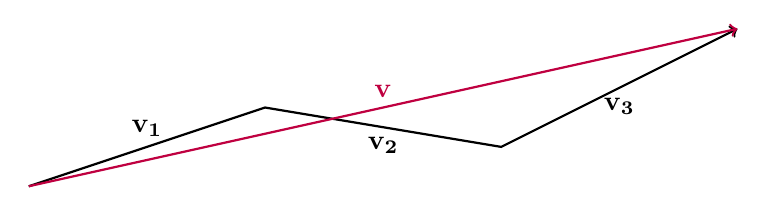
\begin{tikzpicture}
	\draw[thick,->] (0,0) -- node[above] {$\mathbf{v_1}$} (3,1) -- node[below] {$\mathbf{v_2}$} (6,.5) -- node[below] {$\mathbf{v_3}$} (9,2);
	\draw[thick,purple,->] (0,0) -- node[above]{$\mathbf{v}$} (9,2);
	\end{tikzpicture}
	$$\mathbf{v} = \mathbf{v_1}+\mathbf{v_2}+\mathbf{v_3}$$
	\end{center}
\end{figure}

\section{Forces and Accelerations}

\spec{(d) calculate the moment of a force and use the conditions for equilibrium to solve problems (restricted to
	coplanar forces)}

The moment of a force is calculated by multiplying its magnitude by the perpendicular distance of the force's line of action to the pivot point. This is mathematically equivalent to multiplying the distance from the pivot by the component of the force perpendicular to that distance.

\begin{figure}[h]
	\centering
	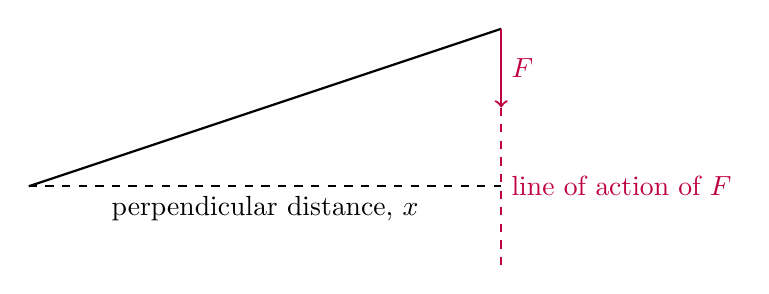
\begin{tikzpicture}
		\draw[thick] (0,0) -- (6,2);
		\draw[thick, purple, ->] (6,2) -- node[right]{$ F$}(6,1);
		\draw[thick, purple, dashed] (6,1) -- node[right] {line of action of $F$}(6,-1) ;
		\draw[thick, dashed] (0,0) -- node[below]{perpendicular distance, $x$} (6,0);

	\end{tikzpicture}
	$$\mathrm{moment} = Fx $$
\end{figure}

The conditions for equilibrium are:
\begin{enumerate}
	\item The sum of all the forces acting on the object must be zero.
	\item The sum of all the moments on an object must be zero.
\end{enumerate}
\fbox{\begin{minipage}[t]{\textwidth}
	\textbf{Example Question}

	A Tower Crane lifts a load into position. The load has a weight of \SI{4.0e4}{N} and the arm of the crane has a weight of \SI{1.2e5}{N}.

	Calculate the required weight of the counterweight and the force the tower must support. Assume the centre of mass of the arm is at its centre.

	\vspace{1cm}

		\begin{center}
		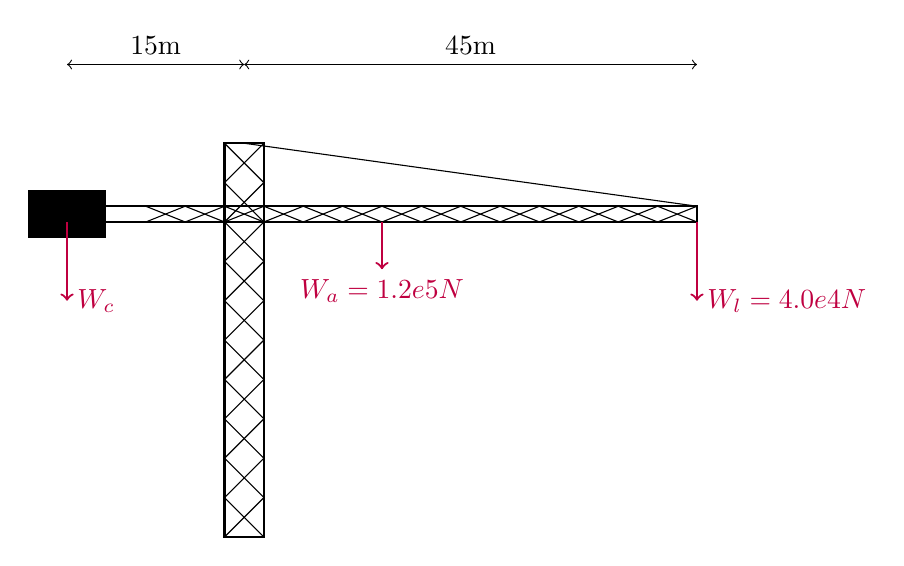
\begin{tikzpicture}
					\draw[thick] (2,0) rectangle (2.5,5);
					\draw[thick] (0,4) rectangle (8,4.2);
					\fill (-0.5,3.8) rectangle (.5,4.4);
					\draw(2.25,5) -- (8,4.2);
					\foreach \x in {0,1,...,13} {
						\draw (1+0.5*\x,4) -- (1.5+0.5*\x,4.2);
						\draw (1+0.5*\x,4.2) -- (1.5+0.5*\x,4);
					}
					\foreach \y in {0,1,...,9} {
						\draw (2,0+0.5*\y) -- (2.5,0.5+0.5*\y);
						\draw (2.5,0+0.5*\y) -- (2,0.5+0.5*\y);
					}
					\draw[purple, thick, ->] (8,4) -- (8,3) node[right]{$W_l=\SI{4.0e4}{N}$};
					\draw[purple, thick, ->] (4,4) -- (4,3.4) node[below]{$W_a=\SI{1.2e5}{N}$};
					\draw[purple, thick, ->] (0,4) -- (0,3) node[right]{$W_c$};
					\draw[<->] (0,6) -- node[above]{15m}(2.25,6);
					\draw[<->] (2.25,6) -- node[above]{45m}(8,6);
				\end{tikzpicture}
		\end{center}

		\textbf{Answer}

		We begin by taking moments around the tower of the crane. The weight of the arm, $W_a$, acts \SI{15}{m} from the tower so solving for moments gives:

		$$ 15W_c = 15W_a + 25W_l $$
		$$ W_c = \SI{4.2e5}{N} $$

		The sum of the downward forces must equal the reaction force of the tower so:

		$$ R = \SI{4.0e5}{N} $$
\end{minipage}}

\spec{(e) construct displacement-time and velocity-time graphs for uniformly accelerated motion}

For uniform acceleration, a graph of velocity against time will be linear, with the formula $ v=u+at$, and a graph of displacement against time will be parabolic, with the formula $s=ut+\frac{1}{2}at^2$.

\begin{center}
	\begin{tikzpicture}[domain=0:3]
		\draw[thick,->] (0,0) -- (3,0) node[below]{$t$};
		\draw[thick,->] (0,0) -- (0,3) node[left]{$s$};
		\draw[thick,->] (4,0) -- (7,0) node[below]{$t$};
		\draw[thick,->] (4,0) -- (4,3) node[left]{$v$};
		\draw[color=purple] plot (\x+4,{.2+0.4*\x});
		\draw[color=purple] plot (\x,{.2*\x+0.2*\x^2});
	\end{tikzpicture}
\end{center}

\spec{(f) identify and use the physical quantities derived from the gradients of displacement-time and areas and
gradients of velocity-time graphs, including cases of non-uniform acceleration}

The quantities are given in the table below:

\begin{tabular}{r|ll}
	& gradient & area  \\ \hline
	displacement-time & velocity & -- \\
	velocity-time & acceleration & displacement \\
\end{tabular}

If the graph is non-linear then the gradient of a tangent must be taken. Note that areas below the axis in a velocity-time graph represent \emph{negative} displacement.

\spec{(g) recall and use:}
\begin{align*}
	v &= \frac{\Delta x}{\Delta t}\\
	a &= \frac{\Delta v}{\Delta t}
\end{align*}

\spec{(h) recognise and use the kinematic equations for motion in one dimension with constant acceleration:}
\begin{align*}
	s &= ut + \frac{1}{2}at^2 \\
	v^2 &= u^2 + 2as \\ s &= \left( \frac{u+v}{2} \right) t
\end{align*}

\spec{(i) recognise and make use of the independence of vertical and horizontal motion of a projectile moving freely under gravity}

When an object moves in a uniform gravitational field it motion can be modelled by considering the horitzontal and vertical components of motion separately. The horizontal component has a constant velocity and the vertical has a constant acceleration.

\fbox{\begin{minipage}[t]{\textwidth}
	\textbf{Example Question}

	A ball is thrown with a velocity of \SI{5}{m.s^{-1}} from a height of \SI{1.2}{m}. If its initial angle to the horizonal is \ang{50} calclate the distance it travels before it hits the ground.

	\textbf{Answer}

	The first step is to split the velocity into horizontal and vertical components:
	\begin{align*}
		v_x = 5\cos{50}\\
		v_y = 5\sin{50}
	\end{align*}

	The time for the ball to reach the ground can now be calculated using the vertical motion and the equation $s=ut+\frac{1}{2}at^2$, setting $s = \SI{-1.2}{m}$. This gives $t=\SI{1.02}{s}$.

	Finally, the horizontal distance is calculated using the simple constant velocity formula to give $x=\SI{3.28}{m}$.
\end{minipage}}

\spec{(j) recognise that internal forces on a collection of objects sum to zero vectorially}

This is as a result of Newton's Third Law.

\spec{(k) recall and interpret statements of Newton’s laws of motion}
\begin{enumerate}
	\item An object will remain at rest, or continue at a constant velocity, unless a resultant force acts upon it.
	\item $F=ma$, where $F$ is the vector sum of the forces acting on the body.
	\item For every force of object A acting on object B there exists a force of the same type, of equal magnitude and opposite direction of object B acting on object A.

	\emph{It is important to be able to distinguish the `equal and opposite´ forces which may act on a single object in equillibrium from a Newton's Third Law pair of forces.}
\end{enumerate}

\end{document}
